% Revisiting the prospects of photonic computing in the AI era
% Build: latexmk -xelatex talk.tex
\documentclass[aspectratio=169,10pt]{beamer}
\usetheme[progressbar=none,numbering=fraction,block=fill]{metropolis}

\usepackage{tikz}
\usetikzlibrary{arrows.meta,positioning,calc,shapes.misc}
\usepackage{pgfplots}
\pgfplotsset{compat=1.18}
\usepackage{booktabs}
\usepackage{fontawesome5}
\usepackage{qrcode}
\usepackage{amsmath,amssymb}

% ---------- palette: deep ink for coherent light, amber accent ----------
\definecolor{ink}{HTML}{16263A}
\definecolor{ink2}{HTML}{2E4A6B}
\definecolor{amber}{HTML}{D9821E}
\definecolor{sky}{HTML}{3A8FB7}
\definecolor{mist}{HTML}{EEF2F6}
\definecolor{paper}{HTML}{FFFFFF}
\definecolor{slate}{HTML}{5B6B7A}
\definecolor{moss}{HTML}{6B8F3D}

\setbeamercolor{normal text}{fg=ink,bg=paper}
\setbeamercolor{title separator}{fg=amber}
\setbeamercolor{frametitle}{fg=paper,bg=ink}
\setbeamercolor{alerted text}{fg=amber}
\setbeamercolor{example text}{fg=sky}
\setbeamercolor{block title}{fg=paper,bg=ink2}
\setbeamercolor{block body}{fg=ink,bg=mist}
\setbeamercolor{footline}{fg=slate}
\setbeamerfont{frametitle}{size=\large}
\setbeamerfont{block title}{size=\small}
\setlength{\leftmargini}{1.1em}

\newcommand{\src}[1]{{\scriptsize\color{slate}#1}}
\newcommand{\stat}[2]{{\fontsize{24}{26}\selectfont\color{amber}\textbf{#1}}\\[-1pt]{\scriptsize\color{slate}#2}}


\title{Revisiting the prospects of photonic computing in the AI era}
\subtitle{Programmable photonic meshes, in situ backpropagation, and what changed after 2022}
\author{Sunil Pai}
\institute{Manager, Design Automation, PsiQuantum\\PhD, Stanford University (2022)}
\date{Stanford Photonics Research Conference\\September 14, 2026}

\begin{document}

% =====================================================================
\maketitle
\note{Title. Ten minutes: two on history, three on the paper, three on what changed, two on where meshes go next.}

% =====================================================================
\begin{frame}{The photonic mesh and its applications}
\begin{columns}[T]
\begin{column}{0.56\textwidth}
\begin{center}
% ---- mesh of MZI boxes ----
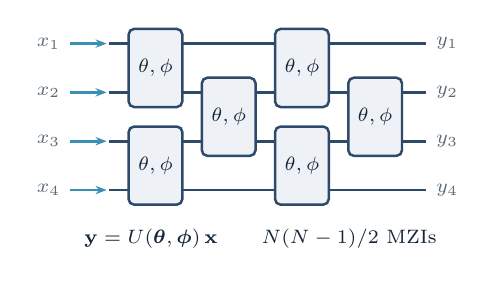
\begin{tikzpicture}[scale=0.62]
  \foreach \y/\lab in {0/4,1/3,2/2,3/1} {
    \draw[ink2,line width=1pt] (-0.2,\y) -- (6.3,\y);
    \draw[-{Stealth[length=4pt]},sky,line width=1pt] (-1.0,\y) -- (-0.25,\y);
    \node[left,font=\scriptsize,color=slate] at (-1.0,\y) {$x_{\lab}$};
    \node[right,font=\scriptsize,color=slate] at (6.3,\y) {$y_{\lab}$};
  }
  \foreach \x/\y in {0.75/0,0.75/2,2.25/1,3.75/0,3.75/2,5.25/1} {
    \draw[ink2,fill=mist,line width=0.9pt,rounded corners=2pt] (\x-0.55,\y-0.3) rectangle (\x+0.55,\y+1.3);
    \node[font=\scriptsize,color=ink] at (\x,\y+0.5) {$\theta,\phi$};
  }
  \node[font=\scriptsize,color=ink] at (2.9,-1.0) {$\mathbf{y} = U(\boldsymbol{\theta},\boldsymbol{\phi})\,\mathbf{x}$\qquad $N(N-1)/2$ MZIs};
\end{tikzpicture}

\vspace{4pt}
% ---- unit cell: phi, coupler, theta, coupler ----
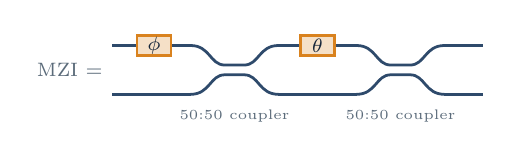
\begin{tikzpicture}[scale=0.62]
  \draw[ink2,line width=1pt] (0,0) -- (1.6,0);
  \draw[ink2,line width=1pt] (0,1) -- (1.6,1);
  % coupler 1
  \draw[ink2,line width=1pt] (1.6,1) .. controls (2.0,1) and (2.0,0.6) .. (2.3,0.6) -- (2.7,0.6) .. controls (3.0,0.6) and (3.0,1) .. (3.4,1);
  \draw[ink2,line width=1pt] (1.6,0) .. controls (2.0,0) and (2.0,0.4) .. (2.3,0.4) -- (2.7,0.4) .. controls (3.0,0.4) and (3.0,0) .. (3.4,0);
  \draw[ink2,line width=1pt] (3.4,0) -- (5.0,0);
  \draw[ink2,line width=1pt] (3.4,1) -- (5.0,1);
  % coupler 2
  \draw[ink2,line width=1pt] (5.0,1) .. controls (5.4,1) and (5.4,0.6) .. (5.7,0.6) -- (6.1,0.6) .. controls (6.4,0.6) and (6.4,1) .. (6.8,1);
  \draw[ink2,line width=1pt] (5.0,0) .. controls (5.4,0) and (5.4,0.4) .. (5.7,0.4) -- (6.1,0.4) .. controls (6.4,0.4) and (6.4,0) .. (6.8,0);
  \draw[ink2,line width=1pt] (6.8,0) -- (7.6,0);
  \draw[ink2,line width=1pt] (6.8,1) -- (7.6,1);
  % phase shifters
  \draw[amber,fill=amber!25,line width=0.9pt] (0.5,0.8) rectangle (1.2,1.2);
  \node[font=\scriptsize,color=ink] at (0.85,1.0) {$\phi$};
  \draw[amber,fill=amber!25,line width=0.9pt] (3.85,0.8) rectangle (4.55,1.2);
  \node[font=\scriptsize,color=ink] at (4.2,1.0) {$\theta$};
  \node[font=\tiny,color=slate] at (2.5,-0.45) {50:50 coupler};
  \node[font=\tiny,color=slate] at (5.9,-0.45) {50:50 coupler};
  \node[left,font=\scriptsize,color=slate] at (0,0.5) {MZI $=$};
\end{tikzpicture}
\end{center}
{\footnotesize Each box is a Mach--Zehnder interferometer: phase $\phi$, a 50:50 coupler, phase $\theta$, a second coupler. A rectangular mesh of them implements \alert{any} $N\times N$ unitary.}
\end{column}
\begin{column}{0.42\textwidth}
{\small
\textbf{Applications}
\begin{itemize}\setlength{\itemsep}{3pt}
  \item \textbf{Universal linear optics} \\ Reck 1994, Clements 2016
  \item \textbf{Self-configuring optics} \\ Miller 2013: mode sorting, unscrambling light, free-space links
  \item \textbf{Quantum photonics} \\ Carolan 2015: reconfigurable interferometers for photons
  \item \textbf{Neural networks} \\ Shen 2017: matrix multiplies for deep learning
  \item \textbf{Programmable photonics} \\ Bogaerts 2020: an FPGA for light
\end{itemize}}
\end{column}
\end{columns}
\note{The mesh is one device with five literatures. Everything in this talk is about the fourth bullet and what it borrowed from the other four.}
\end{frame}

% =====================================================================
\begin{frame}{The 2010s thesis: photonic compute for quantum and AI}
\begin{columns}[T]
\begin{column}{0.48\textwidth}
\begin{block}{Quantum: the mesh \emph{is} the computer}
\footnotesize
\begin{itemize}\setlength{\itemsep}{2pt}
  \item Linear optics, single photons, and detectors are universal (KLM 2001)
  \item Reprogrammable 6-mode universal interferometer on a chip (Carolan et al., \emph{Science} 2015)
  \item Boson sampling, then fusion- and measurement-based architectures built from switches and interferometers
\end{itemize}
\end{block}
\end{column}
\begin{column}{0.48\textwidth}
\begin{block}{AI: the mesh as a matrix engine}
\footnotesize
\begin{itemize}\setlength{\itemsep}{2pt}
  \item Shen et al., \emph{Nat.\ Photonics} 2017: coherent nanophotonic deep learning
  \item Premise: $N^2$ multiply-accumulates per pass for $\mathcal{O}(N)$ conversions and no data movement
  \item Training energy doubling every few months; a digital MAC costs $\approx$ 100 fJ
\end{itemize}
\end{block}
\end{column}
\end{columns}
\vspace{2pt}
\begin{center}
{\small Well over \alert{\$1B} of venture funding followed the AI thesis between 2017 and 2023.}\\[4pt]
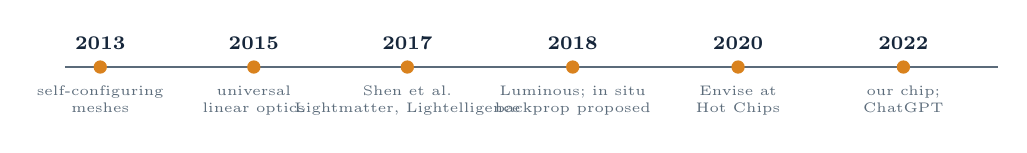
\begin{tikzpicture}[x=1.5cm]
  \draw[slate,line width=1pt] (-0.3,0) -- (7.6,0);
  \foreach \x/\yr/\txt in {0/2013/{self-configuring\\meshes},1.3/2015/{universal\\linear optics},2.6/2017/{Shen et al.\\Lightmatter, Lightelligence},4.0/2018/{Luminous; in situ\\backprop proposed},5.4/2020/{Envise at\\Hot Chips},6.8/2022/{our chip;\\ChatGPT}} {
    \fill[amber] (\x,0) circle (2.4pt);
    \node[above,font=\scriptsize\bfseries,color=ink] at (\x,0.1) {\yr};
    \node[below,font=\tiny,color=slate,align=center] at (\x,-0.12) {\txt};
  }
\end{tikzpicture}
\end{center}
\note{Two communities adopted the same hardware for opposite reasons. Quantum needs the mesh to be exact. AI needs it to be cheap. Keep that tension in mind.}
\end{frame}

% =====================================================================
\begin{frame}{The post-GPT thesis: photonic interconnects}
\begin{columns}[T]
\begin{column}{0.52\textwidth}
{\footnotesize
\textbf{Where the bottleneck went}
\begin{itemize}\setlength{\itemsep}{2pt}
  \item Transformer decode is memory-bandwidth bound: GPUs wait on HBM and on each other
  \item Models grew 100$\times$+, clusters 10$\times$, electrical I/O about 2$\times$
  \item Co-packaged optics replaces pluggables: Nvidia photonic switches (2025), TSMC COUPE, Broadcom
  \item The AI datacenter adopted photonics for \alert{moving} numbers, not multiplying them
\end{itemize}
\vspace{3pt}
\textbf{The best-funded mesh company followed}
\begin{itemize}\setlength{\itemsep}{2pt}
  \item 2021: Passage interconnect announced beside Envise
  \item 2024: \$400M Series D at \$4.4B, for interconnect
  \item 2025: M1000 ships in March; Envise appears in \emph{Nature} in April, as research
\end{itemize}}
\end{column}
\begin{column}{0.44\textwidth}
\begin{center}
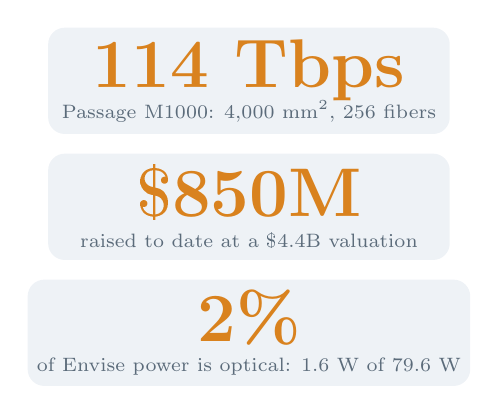
\begin{tikzpicture}
  \node[fill=mist,rounded corners=6pt,minimum width=5.1cm,minimum height=1.35cm,align=center] at (0,0) {\stat{114 Tbps}{Passage M1000: 4,000 mm$^2$, 256 fibers}};
  \node[fill=mist,rounded corners=6pt,minimum width=5.1cm,minimum height=1.35cm,align=center] at (0,-1.6) {\stat{\$850M}{raised to date at a \$4.4B valuation}};
  \node[fill=mist,rounded corners=6pt,minimum width=5.1cm,minimum height=1.35cm,align=center] at (0,-3.2) {\stat{2\%}{of Envise power is optical: 1.6 W of 79.6 W}};
\end{tikzpicture}
\end{center}
\vspace{-2pt}
\src{Lightmatter press and blog, 2024--25; Ahmed et al., \emph{Nature} 640, 368 (2025).}
\end{column}
\end{columns}
\note{The last stat is the pivot in one number. It comes from their own Nature paper. The photons were never the power problem.}
\end{frame}

% =====================================================================
\begin{frame}{Optical neural network theory}
\begin{columns}[T]
\begin{column}{0.52\textwidth}
{\small
\textbf{A layer is a mesh plus a nonlinearity}
\vspace{-4pt}
\[
\mathbf{x}^{(\ell+1)} = f\!\left(M^{(\ell)}\mathbf{x}^{(\ell)}\right),\qquad
M = V\,\Sigma\,U^{\dagger}
\]
\vspace{-8pt}

Any weight matrix is two unitaries and a diagonal of attenuators, so two meshes per layer suffice. One MZI is a 2$\times$2 unitary $T(\theta,\phi)$; $N(N-1)/2$ of them in a grid reach all of $\mathrm{U}(N)$ (Reck 1994; Clements 2016).

\vspace{4pt}
\textbf{Where the energy goes, per multiply-accumulate}
\vspace{-4pt}
\[
E_{\mathrm{MAC}} \approx \underbrace{\frac{E_{\mathrm{DAC}}+E_{\mathrm{ADC}}}{N}}_{\text{conversions}}
+\underbrace{\frac{2^{2b}\,\hbar\omega}{\eta\,N}}_{\text{photons, } b \text{ bits}}
+\underbrace{\frac{P_{\mathrm{hold}}}{f_{\mathrm{clk}}\,N}}_{\text{holding phases}}
\]
}
\end{column}
\begin{column}{0.46\textwidth}
{\footnotesize
\textbf{What the scaling says}
\begin{itemize}\setlength{\itemsep}{3pt}
  \item Every term falls as $1/N$: the mesh pays off only when it is \alert{wide}
  \item Photons are cheap: $10^{5}$ photons per 8-bit detection is well under a femtojoule per MAC
  \item Conversions are not: a GS/s 8-bit ADC costs picojoules, so $N$ must reach the hundreds
  \item Footprint caps $N$ near 64 to 256 per reticle, and error and loss compound over $N$ stages
\end{itemize}
\vspace{2pt}
\begin{block}{The bet}
\footnotesize Optics wins if fan-in $N$ is large, precision $b$ is low, weights change slowly, and the data is already analog. In 2017, none of those described an AI workload.
\end{block}}
\end{column}
\end{columns}
\note{The equation is the whole talk. Three terms, all over N. Hold that thought for the ``what changed'' slide, because two of the four conditions in the box flipped after 2022.}
\end{frame}

% =====================================================================
\begin{frame}{In situ backpropagation and inverse design}
\begin{columns}[T]
\begin{column}{0.47\textwidth}
\begin{center}
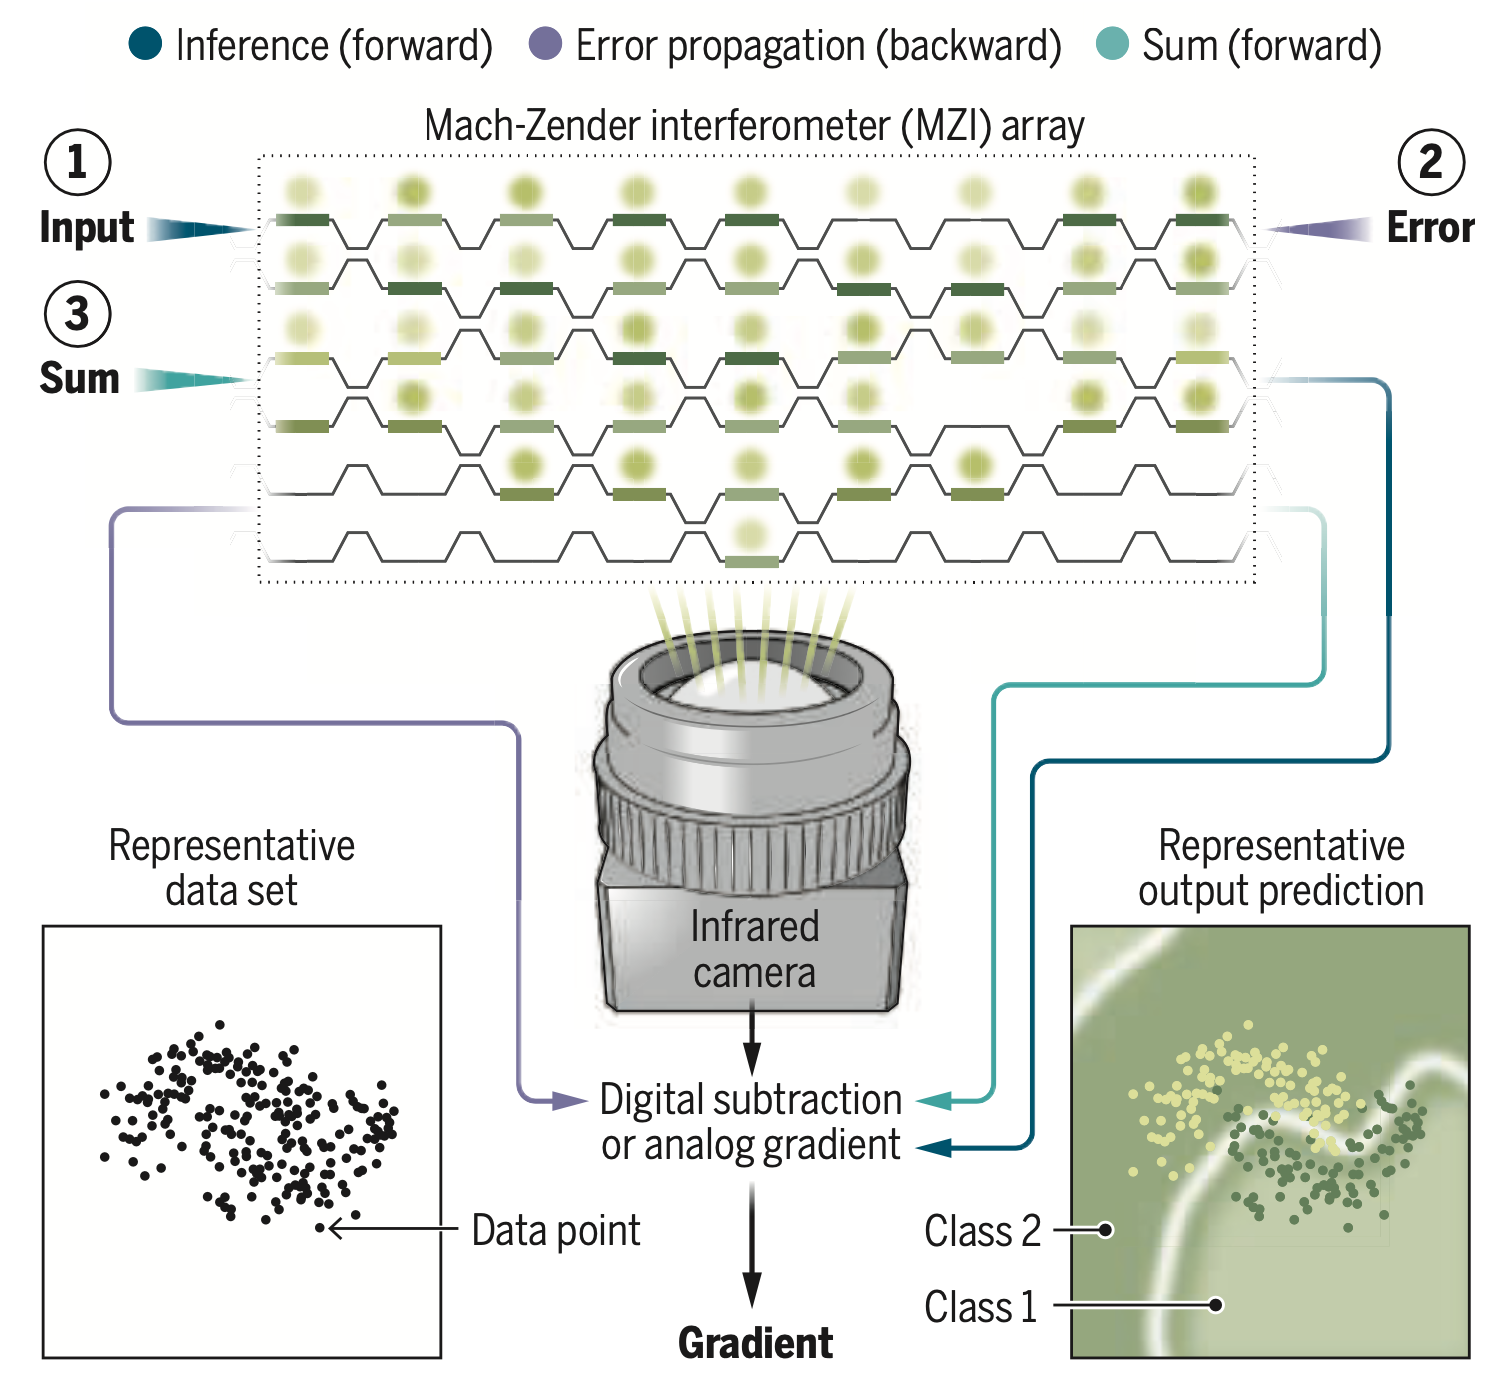
\includegraphics[height=0.66\textheight]{figs/bp.png}
\end{center}
\vspace{-4pt}
\src{Figure: \emph{Science} perspective on Pai et al., \emph{Science} 380, 398 (2023).}
\end{column}
\begin{column}{0.51\textwidth}
{\footnotesize
\textbf{Same trick as photonic inverse design}
\begin{itemize}\setlength{\itemsep}{2pt}
  \item Adjoint method: a gradient is the interference of a forward and a backward field (Hughes, Minkov, Fan 2018)
  \item Forward input, backward error, then their sum: tap power at each phase shifter reads out $\partial\mathcal{L}/\partial\theta$
\end{itemize}
\vspace{2pt}
\textbf{What the chip did}
\begin{itemize}\setlength{\itemsep}{2pt}
  \item 3-layer, 4-port silicon photonic network with thermal phase shifters and grating taps imaged by an IR camera
  \item \alert{Analog update}: one toggle applies the gradient, with no digital subtraction and no $\mathcal{O}(N^2)$ readback
  \item Ring and moons trained \emph{on chip}: 90 to 98\% test accuracy, tracking digital training curves
  \item Simulated 64$\times$64 MNIST: 97\% ideal, 95\% with tap noise and I/O error
\end{itemize}}
\end{column}
\end{columns}
\note{Point at the three colored paths. Forward, backward, sum. The gradient is a power measurement. This is the same adjoint I used at Google X for inverse design; the chip is just a differentiable physical system.}
\end{frame}

% =====================================================================
\begin{frame}{Inference versus training: the energy budget}
\begin{columns}[T]
\begin{column}{0.5\textwidth}
\begin{center}
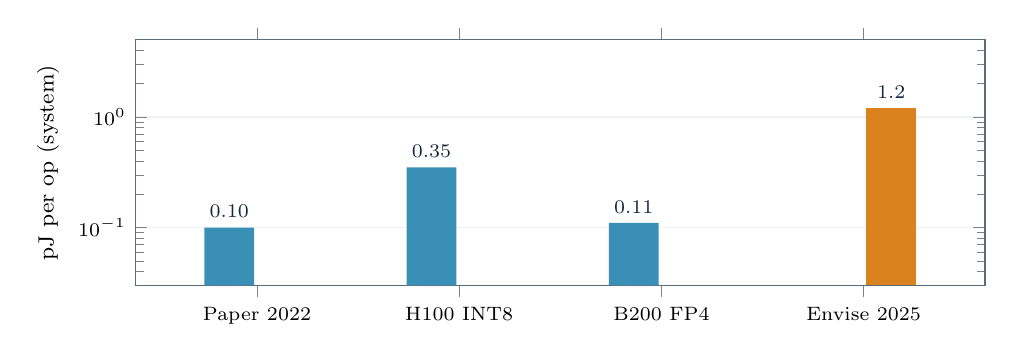
\begin{tikzpicture}
\begin{axis}[
  width=1.02\textwidth, height=4.7cm,
  ybar, bar width=18pt,
  ymode=log, log origin=infty,
  ymin=0.03, ymax=5,
  ylabel={\footnotesize pJ per op (system)},
  ylabel near ticks,
  symbolic x coords={Paper 2022,H100 INT8,B200 FP4,Envise 2025},
  xtick={Paper 2022,H100 INT8,B200 FP4,Envise 2025},
  x tick label style={font=\scriptsize},
  y tick label style={font=\scriptsize},
  ymajorgrids, grid style={color=mist},
  axis line style={color=slate},
  nodes near coords, nodes near coords style={font=\scriptsize,color=ink},
  point meta=explicit symbolic,
  enlarge x limits=0.2,
  clip=false,
]
\addplot[fill=sky,draw=none] coordinates {
  (Paper 2022,0.10) [0.10]
  (H100 INT8,0.35) [0.35]
  (B200 FP4,0.11) [0.11]
};
\addplot[fill=amber,draw=none] coordinates {(Envise 2025,1.2) [1.2]};
\end{axis}
\end{tikzpicture}
\end{center}
\vspace{-6pt}
\src{Digital bars: datasheet peak dense throughput over board power. Envise: 65.5 TOPS at 78 W electrical plus 1.6 W optical (Harris, Apr 2025). Formats differ; read as orders of magnitude.}\\[4pt]
{\footnotesize\textbf{Reading the chart}: a 2025 mesh system sits about 10$\times$ above GPU peak, with 98\% of its power in electronics. The optics are not the term to optimize.}
\end{column}
\begin{column}{0.48\textwidth}
{\footnotesize
\textbf{Inference}: one forward pass
\begin{itemize}\setlength{\itemsep}{2pt}
  \item Tolerates 4 to 8 bits, the analog-friendly regime
  \item Weights static, so phase holding amortizes
  \item Cost is dominated by \alert{conversions}, not photons
\end{itemize}
\vspace{3pt}
\textbf{Training}: forward, backward, update
\begin{itemize}\setlength{\itemsep}{2pt}
  \item Gradients want 16-bit dynamic range, analog's weak spot
  \item In situ backprop: the backward pass is one more optical pass, and the update is $\mathcal{O}(1)$ per phase instead of $\mathcal{O}(N^2)$ memory traffic
  \item But each step rewrites $N^2$ phases, so weight write energy and speed set the budget
\end{itemize}
}
\end{column}
\end{columns}
\note{Be careful with the chart: peak datasheet numbers versus a measured research system. The point is not the ratio, it is which term dominates. In situ training removes the memory traffic term, but it does not touch the conversion term.}
\end{frame}

% =====================================================================
\begin{frame}{What changed after 2022?}
\begin{columns}[T]
\begin{column}{0.48\textwidth}
\begin{block}{Precision collapsed}
\small FP16 in 2017, FP8 with Hopper in 2022, FP4 with Blackwell in 2024. Inference at 4 bits is routine. The industry walked into the regime analog optics always needed.
\end{block}
\begin{block}{Attention moved the bottleneck}
\small Decode is KV-cache and weight-bandwidth bound. Softmax, normalization, and memory traffic are not matrix multiplies. A faster MVM engine attacks the wrong term.
\end{block}
\end{column}
\begin{column}{0.48\textwidth}
\begin{block}{Inference became the product}
\small ChatGPT (Nov 2022), then reasoning models with test-time compute (2024). Inference now dominates deployed FLOPs and spend. Training chips are a market of a few buyers.
\end{block}
\begin{block}{The ADC wall stayed put}
\small Conversion energy per sample improves far slower than logic (Murmann survey). Every photonic accelerator still pays it on every activation, in and out.
\end{block}
\end{column}
\end{columns}
\vspace{6pt}
\begin{center}
{\small Revisit the four conditions: fan-in large \textcolor{slate}{(still hard)}, precision low \textcolor{moss}{\textbf{(now true)}}, weights static \textcolor{moss}{\textbf{(true for inference)}}, data already analog \textcolor{slate}{(not in a datacenter)}.}
\end{center}
\note{Two of the four flipped in our favor. The two that did not are both about where the data lives, which is the hint for the last slide.}
\end{frame}

% =====================================================================
\begin{frame}{Other applications: quantum computing and analog signal processing}
\begin{columns}[T]
\begin{column}{0.48\textwidth}
\begin{block}{Quantum photonics: exactness first}
\footnotesize
\begin{itemize}\setlength{\itemsep}{2pt}
  \item Meshes are the interferometers, switches, and multiplexers of linear-optical quantum computers (Carolan 2015; Xanadu and silicon platforms, \emph{Nature} 2025)
  \item No DAC or ADC in the data path: photons in, detector clicks out
  \item Loss, extinction, and phase accuracy are what matter; accelerator calibration methods transfer directly
\end{itemize}
\end{block}
\end{column}
\begin{column}{0.48\textwidth}
\begin{block}{Analog signal processing and sensing}
\footnotesize
\begin{itemize}\setlength{\itemsep}{2pt}
  \item Mode sorting and unscrambling for free-space and multimode links (Miller 2013; Annoni 2017)
  \item RF photonic filtering and beamforming, lidar wavefront control, optical switching
  \item The signal is already light: conversions only at the boundary, weights updated at kHz by feedback
\end{itemize}
\end{block}
\end{column}
\end{columns}
\vspace{-2pt}
\begin{columns}[c]
\begin{column}{0.36\textwidth}
\begin{center}
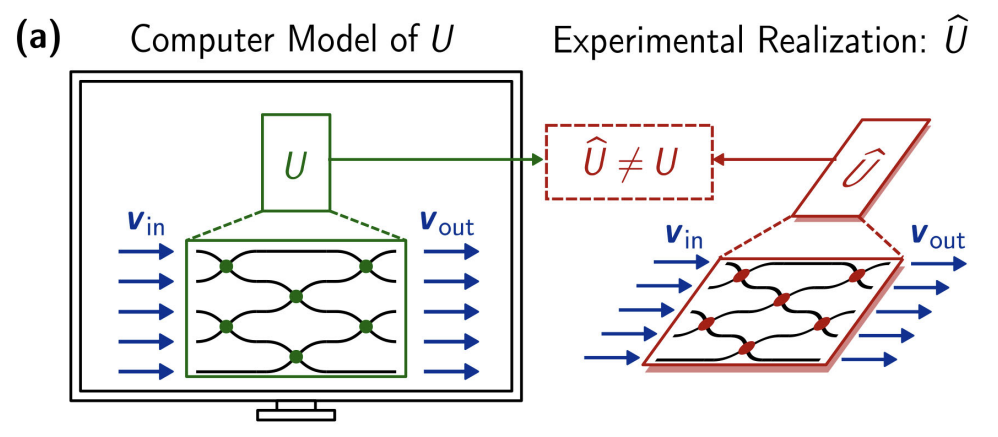
\includegraphics[height=2.2cm]{figs/parallelnull_a.png}
\end{center}
\end{column}
\begin{column}{0.62\textwidth}
{\footnotesize \textbf{The transferable toolkit}: parallel programming of feedforward meshes, power monitoring with two detectors instead of taps, and in situ gradient measurement. Each was built to make an accelerator trustworthy; each is worth more where the mesh \alert{is} the signal path. \src{Pai et al., JSTQE 2020; Nanophotonics 2023; Science 2023.}}
\end{column}
\end{columns}
\note{Do not land a conclusion here. Just show that the same three papers have an obvious home in two fields that never needed the GPU comparison.}
\end{frame}

% =====================================================================
\begin{frame}[standout]
{\LARGE Questions?}\par\vspace{14pt}
\begin{columns}[c]
\begin{column}{0.36\textwidth}
\begin{center}
\qrcode[height=2.6cm]{https://sunilkpai.github.io/blog/}
\end{center}
\end{column}
\begin{column}{0.6\textwidth}
{\normalsize
\faIcon{globe}\; sunilkpai.github.io/blog\\[4pt]
\faIcon{linkedin}\; linkedin.com/in/sunil-pai-96286539\\[4pt]
\faIcon{twitter}\; @sunilkpai\\[4pt]
\faIcon{graduation-cap}\; Google Scholar: Sunil Pai\\[4pt]
\faIcon{envelope}\; sunilkpai93@gmail.com}
\end{column}
\end{columns}
\note{Leave the QR up during questions.}
\end{frame}

\end{document}
